\documentclass[11pt]{article}
\usepackage[a4paper,margin=24mm]{geometry}
\usepackage[T1]{fontenc}
\usepackage{lmodern}
\usepackage{microtype}
\usepackage{amsmath,amssymb,amsthm,mathtools}
\usepackage{bm}
\usepackage{booktabs}
\usepackage{array}
\usepackage{enumitem}
\usepackage{xcolor}
\usepackage{tikz}
\usepackage{hyperref}
\usepackage[capitalize,noabbrev]{cleveref}

\definecolor{deepblue}{RGB}{28,68,128}
\definecolor{deepred}{RGB}{150,50,48}
\definecolor{softgray}{RGB}{244,246,249}
\hypersetup{colorlinks=true,linkcolor=deepblue,citecolor=deepblue,urlcolor=deepblue,
  pdftitle={Two-Query Chirality in Tetrahedral Quantum Echoes},
  pdfauthor={Lluis Eriksson}}
\setlist{nosep,leftmargin=*}
\newtheorem{theorem}{Theorem}[section]
\newtheorem{proposition}[theorem]{Proposition}
\newtheorem{lemma}[theorem]{Lemma}
\newtheorem{corollary}[theorem]{Corollary}
\theoremstyle{definition}
\newtheorem{definition}[theorem]{Definition}
\newtheorem{remark}[theorem]{Remark}
\DeclareMathOperator{\Tr}{Tr}
\DeclareMathOperator{\rank}{rank}
\DeclareMathOperator{\diag}{diag}
\DeclareMathOperator{\spec}{spec}
\DeclareMathOperator{\clamp}{clamp}
\newcommand{\cH}{\mathcal H}
\newcommand{\cO}{\mathcal O}
\newcommand{\cW}{\mathcal W}
\newcommand{\ket}[1]{\lvert #1\rangle}
\newcommand{\bra}[1]{\langle #1\rvert}
\newcommand{\proj}[1]{\lvert #1\rangle\!\langle #1\rvert}

\title{\bfseries Two-Query Chirality in Tetrahedral Quantum Echoes\\[2mm]
\large Exact Parallel Readout, a Nine-Dimensional Query Defect,\\
and a Certified Adaptive Advantage}
\author{Lluis Eriksson}
\date{August 2026}

\begin{document}
\maketitle

\begin{abstract}
Four balanced Pauli kicks along the vertices of a regular tetrahedron, followed
by their reverse echo, generate 24 order-labelled qubit unitary channels.  All
24 words have the same trace and split into two 12-element orbits of the proper
tetrahedral group.  One query sees only the common trace: a Bell tester is
globally optimal and gives the same performance in the two orbit sectors.  We
show that two queries recover information that is invisible at one query.
The quadratic output decomposes as
$\mathbf1\oplus\mathbf2\oplus\mathbf3\oplus\mathbf3$, and two exact chiral
energies $E_\pm$ enter the optimum through a scalar clamp.  This yields closed
formulas for the Bell-square optimum and for the globally optimized parallel
strategy.  The optimal parallel input is generically not two Bell pairs.

At the algebraic pulse point with common half trace $q=1/2$, the parallel value
is
\[
 P_{\rm par}=\frac{5+\sqrt{15}}{24}.
\]
Every causal two-query protocol has success at most $9/24$: fixed trace and
fixed Pauli-vector norm remove one direction from the universal ten-dimensional
quadratic query space.  We give an explicit rational two-comb normalization
and an exact weighted-frame identity attaining this cap.  Hence
\[
 P_{\rm causal}=\frac38>P_{\rm par},\qquad
 P_{\rm causal}-P_{\rm par}=\frac{4-\sqrt{15}}{24}.
\]
This is an analytic adaptive advantage for a non-group unitary ensemble, not a
numerical SDP observation.  A quotient-ring certificate verifies all 24 echo
words, the chiral invariants, the parallel formula, and the causal projector
identity.  A uniform query-norm estimate further proves that the same fixed
adaptive tester beats every parallel tester on an explicit open pulse
interval around the algebraic point.  We make no claim about indefinite
causal order or noisy hardware.
\end{abstract}

\section{Introduction}

Minimum-error discrimination of unitary channels changes qualitatively when
the unknown gate may be queried more than once.  For a uniformly distributed
projective representation of a finite group, covariance often makes parallel
strategies optimal.  Outside the group case, sequential and more general
architectures can be strictly better~\cite{bavaresco2022}.  Explicit analytic
families exhibiting the mechanism remain comparatively scarce: general
tester semidefinite programs certify an optimum, but usually hide why a
particular inter-query memory helps.

This paper gives a closed example derived from a concrete pulse architecture.
Let four control Hamiltonians point to the vertices of a regular tetrahedron.
Executing the four kicks in an order $\sigma\in S_4$ and closing the path by a
reverse echo gives a qubit unitary $W_\sigma$.  The 24 labels do not form a
unitary group.  They form two compound geometrically uniform orbits under
$A_4$, and every word has the same trace.  That common trace makes one-query
readout blind to the difference between the two orbit geometries.  At two
queries, third and fourth moments survive and split the sectors.

The main contributions are as follows.
\begin{enumerate}
\item We derive the complete two-copy representation reduction.  Two
  architecture-specific invariants $E_+$ and $E_-$ are explicit rational
  functions of the pulse parameter.  They determine the exact Bell-square
  optimum by a one-dimensional clamp.
\item We optimize over every parallel input, including arbitrary ancillas.
  Symmetry reduces the input marginal to a singlet weight $a$, after which the
  remaining optimization is elementary.  At $q=1/2$ the answer is
  $(5+\sqrt{15})/24$, attained at
  $a_*=(5-\sqrt{15})/10$; two Bell pairs are strictly suboptimal.
\item We prove an architecture-specific rank cap.  Any purified causal
  two-query protocol is a fixed linear image of $W_\sigma^{\otimes2}$, whose
  span has dimension at most nine rather than the universal ten.
\item We saturate that cap at $q=1/2$.  An explicit rational deterministic
  comb $\Xi_*$ and two positive orbit weights obey $KCK=K$.  This converts the
  24 effective output states into a scalable tight frame and proves the exact
  causal optimum $3/8$.
\item The separation is not confined to one isolated pulse.  A uniform
  Lipschitz estimate gives an explicit interval on which the same adaptive
  tester remains better than the globally optimal parallel strategy.
\end{enumerate}

The ingredients surrounding the result are classical: group-covariant state
discrimination~\cite{eldarforney2001,eldarmegretski2004,krovi2015}, quantum
testers~\cite{chiribella2008,jencova2016}, and unitary-design dimension
bounds~\cite{gross2007,bavaresco2022}.  The new point is their exact synthesis
for this fixed-trace, two-orbit echo family, including a rational adaptive
certificate and a strict closed-form parallel-versus-causal separation.  The
tetrahedral word itself is rederived below, so the argument is logically
self-contained.  The appendices give the full block reduction, a six-Kraus
realization of the inter-query map, and the collision-elimination and
certificate details that are easy to obscure in a short presentation.

\begin{table}[t]
\centering
\small
\caption{Scope of the exact results.  ``Causal'' includes parallel,
sequential, and adaptive two-query circuits with delayed final measurement.}
\begin{tabular}{@{}p{0.25\linewidth}p{0.28\linewidth}p{0.36\linewidth}@{}}
\toprule
Task & Result here & Limitation \\
\midrule
One query, 12 or 24 labels & Exact global tester optimum & Recalled as baseline \\
Two queries, Bell-square & Exact for every pulse & Bell-square is not globally parallel-optimal \\
Two queries, parallel & Exact for every pulse & Formula concerns noiseless channels \\
Two queries, causal & Exact at $q=1/2$; strict advantage on an explicit interval & Rank cap, not full causal optimum, away from $q=1/2$ \\
Collision classification & Exact on the fundamental interval & Labels and channels distinguished \\
\bottomrule
\end{tabular}
\end{table}

\section{The tetrahedral echo family}

Let
\[
r_1=(1,1,1),\quad r_2=(1,-1,-1),\quad
r_3=(-1,1,-1),\quad r_4=(-1,-1,1).
\]
Then $r_a\cdot r_a=3$, $r_a\cdot r_b=-1$ for $a\ne b$, and
$\sum_a r_a=0$.  With the Pauli vector $\bm\sigma$, define
\[
 K_a(y)=\exp[-iy r_a\cdot\bm\sigma]
       =cI-is r_a\cdot\bm\sigma,
 \quad c=\cos(\sqrt3y),\quad
 s=\frac{\sin(\sqrt3y)}{\sqrt3},
\]
so $c^2+3s^2=1$.  The first entry of an order acts first:
\[
 U_\sigma=K_{\sigma_4}K_{\sigma_3}K_{\sigma_2}K_{\sigma_1},
 \qquad
 W_\sigma=U_\sigma U_{\sigma^R}^*.
\]
Equivalently,
\[
 W_\sigma=K_{\sigma_4}(y)\cdots K_{\sigma_1}(y)
 K_{\sigma_4}(-y)\cdots K_{\sigma_1}(-y).
\]
Write
\[
 W_\sigma=q_\sigma I-i v_\sigma\cdot\bm\sigma,
 \qquad q_\sigma^2+\lVert v_\sigma\rVert^2=1.
\]

\begin{proposition}[Common half trace]
For every $\sigma\in S_4$, $q_\sigma=q$, where, with $z=s^2$,
\begin{equation}\label{eq:qpoly}
 q(z)=1-32z^2+128z^3-256z^4,
 \qquad 0\le z\le\frac13.
\end{equation}
The even and odd permutations form two free 12-label orbits
$\cO_+$ and $\cO_-$ under left multiplication by $A_4$.
\end{proposition}

\begin{proof}
If a partial product is $aI-i b\cdot\bm\sigma$, left multiplication by
$cI-isr\cdot\bm\sigma$ sends
\[
 (a,b)\longmapsto(ca-sr\cdot b,\;cb+sar+s r\times b).
\]
Eight iterations for one representative of either parity give the common
scalar
\[
 (c^2-s^2)(c^6+13c^4s^2+35c^2s^4+79s^6).
\]
Substituting $c^2=1-3s^2$ gives \cref{eq:qpoly}.  Proper tetrahedral
rotations act as $A_4$ on labels and conjugate the corresponding words, so one
representative per parity suffices.  The verifier independently expands all
24 words.
\end{proof}

Set $r^2=1-q^2$.  Irreducibility of the real tetrahedral representation gives
for each parity
\begin{equation}\label{eq:mom2}
 \sum_{\sigma\in\cO_\pm}v_\sigma=0,
 \qquad
 \sum_{\sigma\in\cO_\pm}v_\sigma v_\sigma^{\mathsf T}
 =4r^2 I_3.
\end{equation}
These second moments coincide.  The two orbits first separate in higher
moments.

It is useful to replace $z$ by
\[
 t=\frac{c}{s}=\sqrt{\frac{1-3z}{z}}.
\]
The endpoint $z=0$ is understood as $t\to\infty$.  Define the off-diagonal
quadratic energies
\begin{align}
E_+(t)&=\frac{32768(t-1)^8(t+1)^2
 (t^5-t^4+8t^3-8t^2+15t+1)^2}{(t^2+3)^{16}},\label{eq:Eplus}\\
E_-(t)&=\frac{32768(t-1)^2(t+1)^8
 (t^5+t^4+8t^3+8t^2+15t-1)^2}{(t^2+3)^{16}}.\label{eq:Eminus}
\end{align}
For a seed vector in the indicated orbit,
\[
 E_\pm=2\sum_{a<b}v_a^2v_b^2,
 \qquad D_\pm=\frac{2r^4}{3}-E_\pm.
\]
Although \cref{eq:mom2} makes one-query performance identical, the pair
$(D_\pm,E_\pm)$ remembers the orbit.

\section{One query as a symmetry baseline}

Let $\ket\Omega=(\ket{00}+\ket{11})/\sqrt2$ and
$\ket{\psi_\sigma}=(W_\sigma\otimes I)\ket\Omega$.  Vectorization gives
\[
 \langle\psi_\tau|\psi_\sigma\rangle
 =\frac12\Tr(W_\tau^*W_\sigma)
 =q^2+v_\tau\cdot v_\sigma.
\]
For either 12-state orbit, or for their 24-state union with label
multiplicity, the nonzero spectrum of the average state is
\begin{equation}\label{eq:one-spectrum}
 q^2,\qquad \frac{r^2}{3},\quad\frac{r^2}{3},\quad\frac{r^2}{3}.
\end{equation}

Every one-query tester can be symmetrized by $A_4$.  Its input marginal then
commutes with the irreducible two-dimensional spin lift and is therefore
$I_2/2$.  Hence the Bell input loses no performance.  The
Yuen--Kennedy--Lax conditions~\cite{yuen1975} in
$\mathbf1\oplus\mathbf3$ give
\begin{equation}\label{eq:oneuse}
 P_1^{(N)}(q)=
 \frac{\left(|q|+\sqrt{3(1-q^2)}\right)^2}{N},
 \qquad N\in\{12,24\}.
\end{equation}
At $q=\pm1/2$ the four eigenvalues in \cref{eq:one-spectrum} are equal.
Thus a 12-label orbit is a tight frame in dimension four and $P_1^{(12)}=1/3$;
the 24-label value is $1/6$.  This tightness is a one-query statement and does
not imply a unitary two-design.

\section{Two-copy representation and exact Bell-square readout}

For two Bell probes, the normalized output vector is
$\lvert W_\sigma\rangle\!\rangle^{\otimes2}/2$.  The relevant quadratic feature
space is contained in
\[
 \operatorname{Sym}^2(\mathbf1\oplus\mathbf3)
 =\mathbf1^{\oplus2}\oplus\mathbf1'\oplus\mathbf1''
  \oplus\mathbf3^{\oplus2}.
\]
The two invariant coordinates are proportional for every label, leaving one
zero direction.  The two copies of $\mathbf3$ decouple: in coordinates this
is the identity $v\cdot Q(v)=3v_1v_2v_3=0$ on either echo orbit.

\begin{proposition}[Bell-square frame]\label{prop:bellframe}
The average state of the 24 Bell-square outputs has spectrum
\[
 0,\quad m,\quad \lambda_D^{\times2},\quad
 \lambda_V^{\times3},\quad\lambda_E^{\times3},
\]
where
\[
 m=q^4+\frac{r^4}{3},\qquad
 \lambda_D=\frac{D_++D_-}{4},\qquad
 \lambda_V=\frac{2q^2r^2}{3},\qquad
 \lambda_E=\frac{E_++E_-}{6}.
\]
The generic rank is nine.  It is never a tight frame on that support.
\end{proposition}

\begin{proof}
The block eigenvalues follow from Schur averaging and the definitions of
$D_\pm,E_\pm$.  Tightness would in particular require $m=\lambda_V$, or
\[
 6(q^2)^2-4q^2+1=0,
\]
whose discriminant is negative.
\end{proof}

The ensemble is compound geometrically uniform, not a single unitary group.
Consequently the ordinary pretty-good measurement need not be optimal.  The
state-discrimination dual can nevertheless be averaged over $A_4$.  Let
\[
 T=\frac{2r^4}{3},\qquad
 E_c=\clamp\!\left(\frac{2r^4}{5},
 [\min(E_+,E_-),\max(E_+,E_-)]\right),
\]
where $\clamp(x,[u,v])=\min(v,\max(u,x))$, and put
\[
 D_c=T-E_c,\qquad H=\sqrt{2D_c}+\sqrt{3E_c}.
\]

\begin{theorem}[Exact Bell-square optimum]\label{thm:bell2}
For all $z\in[0,1/3]$,
\begin{equation}\label{eq:bell2}
 P_{\mathrm{Bell}^{\otimes2}}
 =\frac1{24}\left(
 \sqrt{q^4+r^4/3}+\sqrt6\,|q|r+H
 \right)^2.
\end{equation}
\end{theorem}

\begin{proof}
Give the $+$ seed constraint dual weight $w\in[0,1]$ and the $-$ seed weight
$1-w$.  Then
$E(w)=wE_++(1-w)E_-$ and $D(w)=T-E(w)$.  Minimizing the positive dual blocks
and using the Schur multiplicities reduces the optimum to
\[
 \frac1{24}\max_{0\le w\le1}
 \left[\sqrt m+\sqrt{2D(w)}+\sqrt{6q^2r^2}
 +\sqrt{3E(w)}\right]^2.
\]
The concave function $\sqrt{2(T-E)}+\sqrt{3E}$ has its unconstrained maximum
at $E=3T/5=2r^4/5$.  Projection to the available interval gives $E_c$.
The corresponding covariant seed operators satisfy the primal completeness
conditions, so the bound is attained.  Appendix~\ref{app:block} gives the
complete isotypic block table, the reduced dual program, and an explicit
attaining primal construction.
\end{proof}

\section{Optimization over every parallel input}

Consider an arbitrary parallel two-query strategy with any retained
reference.  Averaging it over $A_4$ preserves success.  The marginal on the
two queried qubits commutes with the diagonal spin action and therefore has
the form
\begin{equation}\label{eq:rhoa}
 \rho_a=aP_{\rm sing}+\frac{1-a}{3}P_{\rm trip},
 \qquad 0\le a\le1.
\end{equation}
Every such marginal can be purified.  Define
\[
 h=\frac{(4q^2-1)^2}{9},\qquad
 K=\sqrt8\,|q|r+\frac{2H}{\sqrt3}.
\]

\begin{theorem}[Global parallel optimum]\label{thm:parallel}
If $q^2=1$, all labels are the same channel and $P_{\rm par}=1/24$.
Otherwise, for fixed $a$,
\[
 P_{\rm par}(a)=\frac1{24}
 \left[\sqrt{h+(1-h)a}+K\sqrt{1-a}\right]^2.
\]
The optimum over all parallel inputs is
\begin{equation}\label{eq:parallel}
 P_{\rm par}^{\rm opt}=\begin{cases}
 \dfrac1{24}\left(1+\dfrac{K^2}{1-h}\right),
 &hK^2\le(1-h)^2,\\[6pt]
 \dfrac1{24}(\sqrt h+K)^2,&hK^2>(1-h)^2.
 \end{cases}
\end{equation}
In the first branch an attaining singlet weight is
\[
 a_*=1-\frac{K^2}{(1-h)(K^2+1-h)};
\]
in the second branch $a_*=0$.
\end{theorem}

\begin{proof}
In the purification of \cref{eq:rhoa}, the scalar block has squared norm
$h+(1-h)a$.  Every non-scalar block in \cref{thm:bell2} scales by $1-a$.
The same reduced primal-dual calculation therefore gives the displayed
$P_{\rm par}(a)$.  Put $u=\sqrt{(1-h)(1-a)}$.  The bracket becomes
\[
 \sqrt{1-u^2}+\frac{K}{\sqrt{1-h}}u,
 \qquad 0\le u\le\sqrt{1-h}.
\]
Maximizing this planar inner product gives the two branches and $a_*$.  The
symmetrization, purification, and block rescaling are derived explicitly in
Appendix~\ref{app:parallel}.
\end{proof}

Let $z_*$ be the unique root in $(0,1/3)$ of $q(z)=1/2$:
\[
 z_*=0.167964937759754\ldots,\qquad
 y_*=\frac1{\sqrt3}\arcsin\sqrt{3z_*}
     =0.455698535295322\ldots.
\]
At this point the clamp is interior and \cref{eq:parallel} simplifies.

\begin{corollary}[Non-Bell optimum at the tight one-query point]
At $q=1/2$,
\begin{equation}\label{eq:parroot}
 P_{\rm par}^{\rm opt}=\frac{5+\sqrt{15}}{24}
 =0.369707639425309\ldots,\qquad
 a_*=\frac{5-\sqrt{15}}{10}.
\end{equation}
Thus two Bell pairs are not the optimal parallel input, despite a Bell input
being globally optimal for one query.
\end{corollary}

\section{The nine-dimensional causal cap}

The universal two-query dimension bound for qubit unitaries uses
$\dim\operatorname{Sym}^2(\mathbb C^4)=10$~\cite{bavaresco2022}.  The echo
family lies on a fixed conjugacy class and loses one dimension.

\begin{theorem}[Fixed-trace query defect]\label{thm:rankcap}
For any purified causal protocol using the same unknown $W_\sigma$ twice, the
24 final pure states span a space of dimension at most nine.  Therefore
\begin{equation}\label{eq:causalcap}
 P_{\rm causal}^{(2)}\le\frac9{24}=\frac38.
\end{equation}
\end{theorem}

\begin{proof}
Defer all intermediate measurements and purify every fixed operation.  The
final vector is then a fixed linear image of $W_\sigma\otimes W_\sigma$.  Since
$W_\sigma=qI-i v_\sigma\cdot\bm\sigma$ with common $q$ and common
$\lVert v_\sigma\rVert^2=r^2$, its quadratic coordinates consist of one
scalar, three coordinates $qv_a$, and six symmetric products $v_av_b$.
The trace relation $\sum_a v_a^2=r^2$ removes one of these ten directions.
Thus the final span has dimension at most $1+3+5=9$, independently of the
intermediate memory.  For $N$ equiprobable pure hypotheses supported in
dimension $d$, the dual operator $I_d/N$ gives $P\le d/N$.
\end{proof}

The bound is stronger than the universal $10/24$ cap, but a dimension bound
need not be attainable.  We now exhibit exact attainment.

\section{An exact adaptive certificate at \texorpdfstring{$q=1/2$}{q=1/2}}

Use the Choi ordering $B_2A_2B_1A_1$, and let the deterministic two-comb
normalization act on $A_2B_1A_1$.  In the computational basis define
\begin{equation}\label{eq:Xi}
\Xi_*=\frac1{54}\begin{pmatrix}
12&0&0&0&0&0&-8&0\\
0&7&0&0&5&0&0&-8\\
0&0&20&0&0&0&0&0\\
0&0&0&15&0&0&5&0\\
0&5&0&0&15&0&0&0\\
0&0&0&0&0&20&0&0\\
-8&0&0&5&0&0&7&0\\
0&-8&0&0&0&0&0&12
\end{pmatrix}.
\end{equation}
Its spectrum and normalization are
\begin{equation}\label{eq:Xispec}
 \spec(\Xi_*)=\left\{0^{\times2},(7/27)^{\times2},
 (10/27)^{\times4}\right\},
 \qquad
 \Tr_{A_2}\Xi_*=I_{B_1A_1}/2.
\end{equation}
Thus $\Xi_*$ is a valid deterministic causal normalization with maximally
mixed first input.  The realization theorem for quantum combs then identifies
these positive normalization constraints with a causally ordered two-slot
circuit, with the final measurement postponed to the end~\cite{chiribella2009}.
Appendix~\ref{app:kraus} supplies a six-Kraus channel and its Stinespring
implementation, making this comb realization constructive.

Let $t_*>0$ be the unique positive root
\begin{equation}\label{eq:tpoly}
 f(t)=t^8+12t^6-10t^4-20t^2-239=0.
\end{equation}
This is exactly the $q=1/2$ condition.  Put
\[
 \ket{J_\sigma^{(2)}}=\lvert W_\sigma\rangle\!\rangle^{\otimes2},
 \qquad
 K_{\sigma\tau}=\bra{J_\sigma^{(2)}}
 (I_{B_2}\otimes\Xi_*)\ket{J_\tau^{(2)}}.
\]
All diagonal entries of $K$ equal one.  Define the field element
\[
 \delta(t)=-\frac{t(27686401t^6+85868681t^4
 -2778560421t^2+1179263131)}{34125376000}.
\]
At $t=t_*$ set
\begin{equation}\label{eq:cweights}
 c_+=\frac38-\delta(t_*),\qquad
 c_-=\frac38+\delta(t_*).
\end{equation}
Numerically,
\begin{align*}
 c_+&=0.09473473348\ldots,&
 c_-&=0.65526526651\ldots.
\end{align*}
In particular both weights are strictly positive.  Let
$C=\diag(c_+I_{12},c_-I_{12})$, with labels ordered by parity.

\begin{lemma}[Exact scalable-frame identity]\label{lem:KCK}
At the algebraic point \cref{eq:tpoly},
\begin{equation}\label{eq:KCK}
 KCK=K,\qquad 12(c_++c_-)=9.
\end{equation}
\end{lemma}

\begin{proof}
Write every pulse as
$(tI-ir_a\cdot\bm\sigma)/\sqrt{t^2+3}$.  Each echo entry is then a rational
function with denominator $(t^2+3)^4$.  Hence every entry of $KCK-K$ belongs
to $\mathbb Q(t)$ with denominator nonzero at $t_*$.  Reducing the 576
numerators modulo $f(t)$ gives zero.  By $A_4$ covariance it is enough to
check one row representative from each parity orbit.  Positivity of $c_\pm$
follows by rational interval evaluation on the isolating interval
$1.71860<t_*<1.71862$.  The accompanying verifier performs these quotient-ring
operations directly; no floating-point SDP is used.
\end{proof}

\begin{theorem}[Exact adaptive advantage]\label{thm:adaptive}
At $q=1/2$, the optimal success probability among all causally ordered
two-query protocols is
\begin{equation}\label{eq:causalexact}
 P_{\rm causal}^{(2)}=\frac38.
\end{equation}
It strictly exceeds the global parallel optimum:
\begin{equation}\label{eq:gain}
 P_{\rm causal}^{(2)}-P_{\rm par}^{\rm opt}
 =\frac{4-\sqrt{15}}{24}>0.
\end{equation}
\end{theorem}

\begin{proof}
Let $\ket{\phi_\sigma}$ be the normalized effective state obtained by applying
$I\otimes\Xi_*^{1/2}$ to $\ket{J_\sigma^{(2)}}$.  Its Gram matrix is $K$.
Define
\[
 M_\sigma=c_\pm\proj{\phi_\sigma},
 \qquad \sigma\in\cO_\pm.
\]
The identity $KCK=K$ says that
$\sum_\sigma M_\sigma$ is the orthogonal projector onto the span of the
effective states.  Complete it arbitrarily on the unused orthogonal
complement.  This gives a valid final POVM for the deterministic comb
$\Xi_*$.  Its success is
\[
 \frac1{24}\sum_\sigma c_\pm
 |\langle\phi_\sigma|\phi_\sigma\rangle|^2
 =\frac{12(c_++c_-)}{24}=\frac38.
\]
The upper bound is \cref{thm:rankcap}; hence the strategy is optimal.  Subtract
\cref{eq:parroot} to obtain \cref{eq:gain}.
\end{proof}

The exact point also forces an open interval of adaptive advantage.  This is
useful because it separates the phenomenon from algebraic fine tuning.

\begin{corollary}[Certified open pulse interval]\label{cor:open}
Let $y_*=0.455698535295322\ldots$ be the pulse in \cref{eq:parroot}.  Keep the
comb and final POVM of \cref{thm:adaptive} fixed while varying the 24 echo
words with $y$.  Then this causal strategy strictly outperforms every
parallel two-query strategy whenever
\begin{equation}\label{eq:openinterval}
 |y-y_*|<\frac{4-\sqrt{15}}{1536\sqrt3}
 =4.7742903163\ldots\times10^{-5}.
\end{equation}
Consequently the optimal causal value is strictly larger than the parallel
optimum throughout that interval.
\end{corollary}

\begin{proof}
Each echo is a product of eight factors whose Hermitian generators have norm
$\sqrt3$, hence $\lVert W_\sigma'(y)\rVert\le8\sqrt3$.  After two queries,
the derivative of any normalized purified output has norm at most
$16\sqrt3$.  Therefore the success probability of any fixed tester is
$32\sqrt3$-Lipschitz.  Taking the supremum preserves the same constant, so
$P_{\rm par}^{\rm opt}(y)$ is also $32\sqrt3$-Lipschitz.  The difference
between the fixed causal strategy and the parallel optimum can thus decrease
from its value $(4-\sqrt{15})/24$ at speed at most $64\sqrt3$.  The radius in
\cref{eq:openinterval} follows.
\end{proof}

This separation does not follow from the standard parallelization results.
Those results cover binary unitary sequences or covariant estimation when the
queried unitaries form a group representation~\cite{chiribella2008}; the 24
echo words here form two conjugacy orbits and are not closed under
multiplication.  Non-group ensembles can exhibit a sequential advantage in
general~\cite{bavaresco2022}, but that fact supplies neither the value nor a
strategy for this family.  Equations~\eqref{eq:Xi}--\eqref{eq:KCK} provide the
missing architecture-specific certificate.

\begin{figure}[t]
\centering
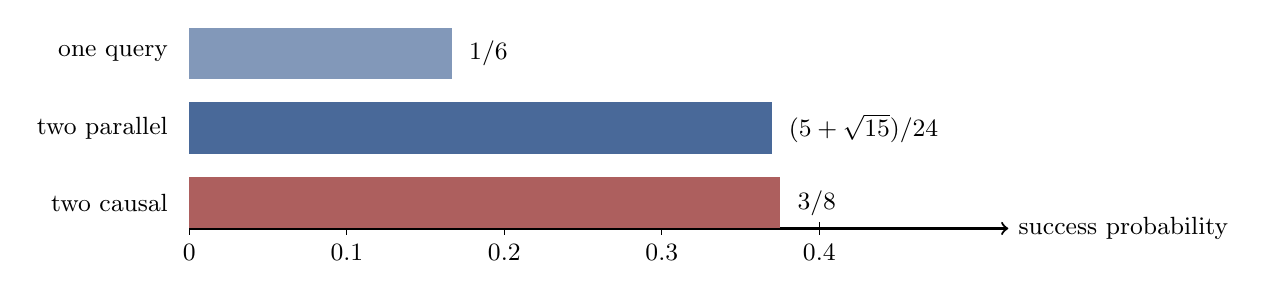
\begin{tikzpicture}[x=1cm,y=1cm,font=\small]
  \draw[->,thick] (0,0)--(10.4,0) node[right] {success probability};
  \foreach \x/\lab in {0/0,2/0.1,4/0.2,6/0.3,8/0.4}
    {\draw (\x,0.08)--(\x,-0.08) node[below] {\lab};}
  \fill[deepblue!55] (0,1.9) rectangle (3.3333,2.55);
  \fill[deepblue!80] (0,0.95) rectangle (7.39415,1.60);
  \fill[deepred!78] (0,0) rectangle (7.5,0.65);
  \node[anchor=east] at (-0.15,2.22) {one query};
  \node[anchor=east] at (-0.15,1.27) {two parallel};
  \node[anchor=east] at (-0.15,0.32) {two causal};
  \node[anchor=west] at (3.43,2.22) {$1/6$};
  \node[anchor=west] at (7.49,1.27) {$(5+\sqrt{15})/24$};
  \node[anchor=west] at (7.60,0.32) {$3/8$};
\end{tikzpicture}
\caption{Exact values for 24 labelled orders at $q=1/2$.  The second use
more than doubles the one-query success, and causal memory gives the strict
gain $(4-\sqrt{15})/24$ over every parallel input.}
\label{fig:values}
\end{figure}

\section{Channel collisions and interpretation}

The discrimination problem is label-valued.  At exceptional pulses, distinct
labels can implement the same $SU(2)$ word, and $W$ and $-W$ define the same
physical channel.  On the fundamental branch $0\le z\le1/3$, all exact word
collisions occur at four points:
\begin{center}
\begin{tabular}{@{}lll@{}}
\toprule
Pulse point & $SU(2)$ word classes & Physical channel classes \\
\midrule
$z=0$ & one class of size 24 & one class of size 24 \\
$z=1/4$ & six classes of size 4 & three classes of size 8 \\
$64z^3-4z-1=0$ & twelve classes of size 2 & same twelve classes \\
$256z^5-64z^4-16z^3+12z^2-1=0$ & six pairs and twelve singles & same 18 classes \\
generic $z$ & 24 singles & 24 singles \\
\bottomrule
\end{tabular}
\end{center}
The point $z_*$ used in \cref{thm:adaptive} is generic, so its 24 physical
channels are distinct.  Appendix~\ref{app:certificate} proves completeness of
the table by resultants, Sturm isolation, and direct projective filtering.

The operational phenomenon can now be stated precisely.  A single query
depends only on the second moments \cref{eq:mom2}, and therefore only on the
common scalar $q$.  Two queries expose $E_+-E_-$, a higher-order orbit
invariant.  The causal comb \cref{eq:Xi} uses the first output coherently when
preparing the second input; it rescales the two orbit frames just enough to
make the nine-dimensional query cap attainable.  This is not causal
nonseparability.  It is an advantage inside ordinary causally ordered quantum
circuits.

\section{Reproducibility and limitations}

The release contains three independent lightweight checks with deliberately
different certification levels.
\begin{enumerate}
\item A word audit expands all 24 eight-pulse echoes symbolically over
  $\mathbb Q[c,s]/(c^2+3s^2-1)$, verifies the common trace, both tetrahedral
  moments, and the collision resultants; numerical root isolation and tolerant
  grouping are used as diagnostics for the physical collision classes.
\item A representation audit checks the two-copy block spectrum, scalar clamp,
  and parallel fixture at $q=1/2$ using NumPy with an explicit tolerance.  The
  all-pulse parallel theorem is established by the analytic block reduction,
  not by this numerical replay.
\item A causal audit works in $\mathbb Q[t]/(f)$ at $q=1/2$.  It verifies
  \cref{eq:Xispec}, reconstructs the 24 effective states, proves positivity of
  $c_\pm$, and reduces every entry of $KCK-K$ to zero.  It then checks the
  exact $3/8$ success and the strict algebraic gap.
\end{enumerate}
Thus the central causal certificate is exact and uses no numerical SDP.  The
other two scripts are transparent corroborating audits, while the universal
parallel reduction and collision completeness remain mathematical proofs in
the text.  The dependency file records both SymPy and NumPy.

Several limitations are deliberate.  We do not optimize indefinite-causal-
order processes.  We do not model pulse noise, finite measurement statistics,
or laboratory compilation cost.  The 24 hypotheses are known implementations
with an unknown label, not an unknown continuous unitary.  Finally, the
dimension-nine obstruction is architecture-specific: it comes from common
trace and norm, and is not asserted for arbitrary qubit ensembles.

\section{Conclusion}

Tetrahedral echo order has a genuinely query-dependent memory.  One query
compresses the two parity orbits to the same $\mathbf1\oplus\mathbf3$
spectrum.  Two queries recover their different quadratic energies, make the
Bell-square input suboptimal, and admit a complete parallel solution.  At the
algebraic point $q=1/2$, a rational causal comb saturates a sharpened
nine-dimensional query bound and strictly outperforms all parallel
architectures.  The resulting separation is exact, analytic, and certified
over all 24 pulse orders.  The explicit neighborhood in
Corollary~\ref{cor:open} shows that the advantage is robust as a mathematical query
phenomenon, even though no laboratory noise model is asserted.

\appendix

\section{The full two-copy block reduction}\label{app:block}

This appendix expands the representation steps used in
\cref{prop:bellframe,thm:bell2,thm:parallel}.
For $x=(q,-iv)\in\mathbf1\oplus\mathbf3$, the symmetric square decomposes
under $A_4$ as
\[
 \operatorname{Sym}^2(\mathbf1\oplus\mathbf3)
 =\mathbf1^{\oplus2}\oplus\mathbf1'\oplus\mathbf1''
  \oplus\mathbf3_V\oplus\mathbf3_E.
\]
The two invariant coordinates are $q^2$ and $-\lVert v\rVert^2/\sqrt3$.
They are proportional for all labels, so only one invariant direction is
occupied.  The first copy of $\mathbf3$ is represented by $qv$.  The second
is represented by
\[
 Q(v)=\sqrt2\,(v_2v_3,v_3v_1,v_1v_2).
\]
A direct recurrence for either parity seed gives $v_1v_2v_3=0$; the proper
tetrahedral rotations are signed coordinate permutations, so the identity
holds on each entire orbit.  Hence
\[
 \langle v,Q(v)\rangle=3\sqrt2\,v_1v_2v_3=0,
\]
and Schur averaging cannot couple $\mathbf3_V$ to $\mathbf3_E$.  This is the
claimed decoupling of the two equivalent three-dimensional summands.

For a seed in orbit $\varepsilon\in\{+,-\}$, the squared block norms are
\begin{center}
\begin{tabular}{@{}ccccc@{}}
\toprule
block & occupied $\mathbf1$ & $\mathbf1'\oplus\mathbf1''$
 & $\mathbf3_V$ & $\mathbf3_E$\\
\midrule
dimension & 1 & 2 & 3 & 3\\
seed norm squared & $m$ & $D_\varepsilon$ & $2q^2r^2$ & $E_\varepsilon$\\
\bottomrule
\end{tabular}
\end{center}
where $m=q^4+r^4/3$ and $D_\varepsilon+E_\varepsilon=2r^4/3$.
This table immediately yields the spectrum in \cref{prop:bellframe}.

For completeness, the reduced minimum-error SDP can also be solved without
suppressing the scalar step.  Let $w\in[0,1]$ be the multiplier of the $+$
seed constraint and write
\[
 E(w)=wE_++(1-w)E_-,\qquad
 D(w)=\frac{2r^4}{3}-E(w).
\]
On a multiplicity-free block of dimension $d$, minimizing a positive scalar
dual block that dominates a rank-one component of squared norm $e$ contributes
$\sqrt{de}$ to the trace square root.  The Schur-complement condition for all
four occupied blocks therefore gives
\begin{equation}\label{eq:reduceddual}
 \frac1{24}\max_{0\le w\le1}
 \left[\sqrt m+\sqrt{2D(w)}+\sqrt6\,|q|r
       +\sqrt{3E(w)}\right]^2.
\end{equation}
The primal has strictly feasible seeds after adding an arbitrarily small
multiple of the identity, so finite-dimensional SDP strong duality applies.
Thus \cref{eq:reduceddual} is not merely an upper bound.  The only variable
term is $\sqrt{2(T-E)}+\sqrt{3E}$ with $T=2r^4/3$.  Its stationary point is
$E=3T/5=2r^4/5$; projecting it onto the interval with endpoints $E_+,E_-$
gives exactly the clamp in \cref{thm:bell2}.

\section{Why one singlet parameter solves every parallel input}\label{app:parallel}

After $A_4$ symmetrization, an arbitrary two-qubit query marginal is
\[
 \rho_a=aP_{\rm sing}+\frac{1-a}{3}P_{\rm trip},\qquad0\le a\le1.
\]
This is exhaustive because the diagonal spin representation is
$\mathbf1\oplus\mathbf3$, with both summands irreducible.  Every $\rho_a$ has
a purification, so optimizing $a$ includes arbitrary retained references.

The singlet is fixed by $W_\sigma\otimes W_\sigma$.  On the triplet, the
normalized invariant overlap is the spin-one character divided by three,
\[
 \eta(q)=\frac{\chi_1(W_\sigma)}3=\frac{4q^2-1}{3},
 \qquad h=\eta(q)^2.
\]
Consequently the occupied scalar block has squared norm
$h+(1-h)a$, while every non-scalar block in \cref{eq:reduceddual} is multiplied
by $1-a$.  Substitution gives, without an ansatz on the reference system,
\[
 P_{\rm par}(a)=\frac1{24}
 \left[\sqrt{h+(1-h)a}+K\sqrt{1-a}\right]^2.
\]
Put $u=\sqrt{(1-h)(1-a)}$.  The bracket becomes
\[
 \sqrt{1-u^2}+\frac{K}{\sqrt{1-h}}u,
 \qquad0\le u\le\sqrt{1-h}.
\]
It is the inner product of $(\sqrt{1-u^2},u)$ with a fixed vector.  The
unconstrained maximizer lies inside the interval exactly when
$hK^2\le(1-h)^2$; otherwise the endpoint $a=0$ is optimal.  This proves both
branches and the stated $a_*$ in \cref{thm:parallel}.  At $q=1/2$, $h=0$ and
the displayed expressions reduce algebraically to \cref{eq:parroot}.

\section{A concrete six-Kraus realization of the causal comb}\label{app:kraus}

The positivity and partial-trace equations in \cref{eq:Xispec} already imply
physical realizability by the comb theorem.  Here is an explicit dilation.
Identify the stored reference with a copy of $A_1$, and use the output-major
vectorization $\lvert L\rangle\!\rangle\in A_2\otimes(B_1A_1)$.  Then
$J(\Lambda)=2\Xi_*$ is the Choi matrix of a channel
$\Lambda:B_1A_1\to A_2$.  One exact Kraus family is
\begin{align*}
L_1&=\frac19\begin{pmatrix}-4&0&0&-5\\0&0&1&0\end{pmatrix},&
L_2&=\frac19\begin{pmatrix}0&-1&0&0\\5&0&0&4\end{pmatrix},\\
L_3&=\frac{2\sqrt{15}}9\begin{pmatrix}0&0&1&0\\0&0&0&0\end{pmatrix},&
L_4&=\frac{2\sqrt{15}}9\begin{pmatrix}0&0&0&0\\0&1&0&0\end{pmatrix},\\
L_5&=\frac{2\sqrt5}9\begin{pmatrix}-1&0&0&1\\0&0&1&0\end{pmatrix},&
L_6&=\frac{2\sqrt5}9\begin{pmatrix}0&-1&0&0\\-1&0&0&1\end{pmatrix}.
\end{align*}
Direct multiplication gives
\[
 \sum_{\mu=1}^6L_\mu^*L_\mu=I_4,
 \qquad
 \sum_{\mu=1}^6\lvert L_\mu\rangle\!\rangle
 \langle\!\langle L_\mu\rvert=2\Xi_*.
\]
Thus a circuit can prepare a Bell purification of the first maximally mixed
input, store its reference, and after receiving $B_1$ apply the Stinespring
isometry
\[
 V=\sum_{\mu=1}^6L_\mu\otimes\ket{\mu}_M.
\]
The $A_2$ output is sent through the second unknown channel and $M$ is retained
for the final measurement.  The orbit-weighted rank-one POVM in the proof of
\cref{thm:adaptive} completes this explicit sequential circuit.  Hence the
attainment is not only an abstract feasible comb matrix.

\section{Collision completeness and replay details}\label{app:certificate}

For each of the 276 unordered label pairs, the word recurrence first computes
$\lVert v_\sigma-v_\tau\rVert^2$ in
$\mathbb Q[c,s]/(c^2+3s^2-1)$.  After setting $z=s^2$, reduction by
$c^2=1-3z$ leaves an expression $A(z)+cB(z)$.  If $B=0$, its roots are tested
directly.  Otherwise every physical root must divide
\[
 A(z)^2-(1-3z)B(z)^2.
\]
Factoring these resultants gives 17 distance types.  Sturm isolation on
$[0,1/3]$, followed by substitution of the physical branch
$c=\sqrt{1-3z}$, removes squared-resultant artifacts and leaves exactly the
four rows of the collision table.  Finally, $W_\sigma=-W_\tau$ is possible
only when the common scalar $q$ vanishes, which adds only the projective
identifications at $z=1/4$.  This proves completeness, rather than merely
discovering candidate collision points numerically.

The supplementary archive contains the manuscript source, manifest, and
three fail-closed scripts:
\begin{verbatim}
python verification/verify_coherent_order_echo.py
python verification/verify_two_use_a4.py
python verification/verify_two_use_causal_qhalf.py
\end{verbatim}
The first performs symbolic 24-word and 276-pair elimination, followed by
numerical root screening and tolerant class grouping.  The second uses NumPy
to check the two-copy spectrum, clamp, and parallel fixture at $q=1/2$.  The
third works in the exact field $\mathbb Q[t]/(f)$, verifies the Kraus/comb
normalization, isolates the physical root, and reduces every numerator of
$KCK-K$ to zero.  Accordingly, only the third is advertised as a fully exact
machine certificate; the first two are reproducible diagnostics supporting
the analytic arguments above.  None invokes an SDP solver or random sample.

\section*{AI assistance disclosure}
AI tools assisted with symbolic exploration, literature triage, code drafting,
and language editing.  The author selected the claims and assumptions.  The
central causal identity is replayed exactly; the remaining scripts provide
symbolic and numerical corroboration at the scopes stated above.  AI output is
not treated as independent evidence.

\bibliographystyle{unsrt}
\bibliography{references}

\end{document}
